\documentclass{article}

% COMP7608B submission: NeurIPS 2026 format, but authors must be visible.
% The course does not require an abstract; therefore none is included.
\usepackage[nonanonymous]{neurips_2026}
\usepackage[T1]{fontenc}
\usepackage[utf8]{inputenc}
\usepackage{microtype}
\usepackage{booktabs}
\usepackage{graphicx}
\usepackage{float}
\usepackage{tabularx}
\usepackage{array}
\usepackage{tikz}
\usetikzlibrary{arrows.meta,positioning,calc,fit}
\usepackage{hyperref}
\hypersetup{hidelinks}

% Suppress the NeurIPS footer notice (course submission, not conference submission).
\makeatletter
\renewcommand{\@notice}{}
\makeatother

\title{KORA: An Agentic Knowledge Assistant\\
for Multi-Step Retrieval and Reasoning}
\author{Group 9}

\begin{document}
\maketitle

\section{Group members}
% A centered, borderless two-by-two group roster matching the approved sample.
\newcommand{\koramember}[3]{%
  \shortstack[c]{\textbf{\normalsize #1}\\[-0.15ex]
  {\footnotesize Student ID: #2}\\[-0.15ex]
  {\scriptsize\texttt{#3}}}%
}
\vspace{-0.2em}
\begin{center}
\begin{tabularx}{\linewidth}{@{}>{\centering\arraybackslash}X >{\centering\arraybackslash}X@{}}
\koramember{Kunhan Guo}{3036086995}{aguo0521@connect.hku.hk} &
\koramember{Tim Lung Lam}{3036653944}{u3665394@connect.hku.hk} \\[1.15em]
\koramember{Yui Hung Leung}{3035689752}{rayhi@connect.hku.hk} &
\koramember{Yutong Yuan}{3036793897}{u3679389@connect.hku.hk}
\end{tabularx}
\end{center}
\vspace{-0.55em}

\section{Project objective}
We propose KORA (Knowledge-Oriented Reasoning Agent), a modular agent that retrieves and connects evidence, chooses tools, plans intermediate actions, and revises its decisions using feedback. The intended long-term application is a knowledge assistant for information-intensive user tasks. Its initial users are data analysts and business users who need to answer natural-language database questions without manually identifying tables, columns, or join paths. In future, the same core could help knowledge workers find and verify information across documents, though this is outside the current evaluation. Rather than committing to multiple applications, this project develops a reusable stateful controller and evaluates one fully runnable instantiation: knowledge-guided Text-to-SQL on BIRD Mini-Dev. Database interaction supplies observable tool feedback and objective end-to-end correctness, while a separate domain adapter preserves the ability to replace SQL-specific tools with document tools in future work.

Our central question is: Which parts of an adaptive knowledge-reasoning workflow improve Text-to-SQL accuracy, recovery, or inference efficiency, and under what conditions? Specifically, we test (i) adaptive tool use against non-agentic workflows, (ii) graph-guided relationship exploration, (iii) explicit query planning, and (iv) cost-aware model selection. KORA follows an iterative reasoning-and-acting approach \citep{yao2023react}; benefits are hypotheses to test, not assumed outcomes.

\section{Motivation and challenges}
Knowledge-intensive questions often require several evidence-gathering steps. In Text-to-SQL, the question ``Which customers purchased a product category but not in the following month?'' may require identifying relevant columns, recovering intermediate join tables, interpreting dates, and constructing an anti-join or exclusion condition. Pure lexical schema matching can overlook these dependencies; even a syntactically valid SQL query may be semantically incorrect. Prior Text-to-SQL work emphasizes relational schema linking \citep{wang2020ratsql}, while BIRD highlights grounding in database contents and supporting knowledge \citep{li2023bird}.

The main challenges are selective discovery (avoid overwhelming the model with full schemas), relationship reasoning (find multi-hop join paths and connect terminology to fields), adaptive recovery (choose a useful next action after incomplete evidence or SQL feedback), and efficient inference (spend stronger-model computation only when justified). The last challenge is related to language-model cascades \citep{chen2023frugalgpt}.

\section{Potential solutions}
\textbf{Reusable KORA core.} A bounded Perceive $\rightarrow$ Decide/Plan $\rightarrow$ Act $\rightarrow$ Observe/Reflect loop maintains the question, retrieved evidence, candidate join paths, draft query plan, SQL attempts, tool observations, and remaining budget. At each step, the controller selects an action from the available tool interface or terminates. A runtime validates actions, executes tools, records observations, and returns updated state. This separates LLM-driven action selection from deterministic execution; LangGraph or an equivalent framework can implement the loop \citep{langchain2026langgraph}.

\begin{figure}[H]
\centering
% Editable reproduction of the original KORA controller and domain-adapter chart.
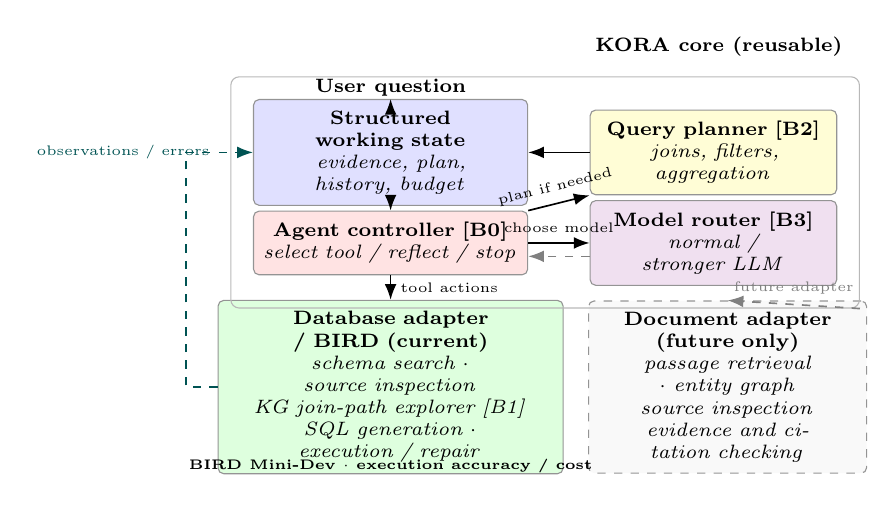
\begin{tikzpicture}[
 >=Latex,font=\scriptsize,
 kbox/.style={draw=black!42,rounded corners=2pt,align=center,minimum height=0.7cm,inner sep=4pt},
 state/.style={kbox,fill=blue!12,text width=3.2cm},
 core/.style={kbox,fill=red!11,text width=3.2cm},
 plan/.style={kbox,fill=yellow!16,text width=2.85cm},
 routing/.style={kbox,fill=violet!12,text width=2.85cm},
 current/.style={kbox,fill=green!13,text width=4.1cm},
 future/.style={kbox,draw=black!42,dashed,fill=gray!5,text width=3.25cm},
 arrow/.style={->,semithick}]
\node (user) at (-2.1,3.95) {\textbf{User question}};
\node[state] (work) at (-2.1,3.13) {\textbf{Structured working state}\\\emph{evidence, plan, history, budget}};
\node[plan] (planner) at (2,3.13) {\textbf{Query planner [B2]}\\\emph{joins, filters, aggregation}};
\node[core] (agent) at (-2.1,1.98) {\textbf{Agent controller [B0]}\\\emph{select tool / reflect / stop}};
\node[routing] (model) at (2,1.98) {\textbf{Model router [B3]}\\\emph{normal / stronger LLM}};
\node[current] (db) at (-2.1,0.15) {\textbf{Database adapter / BIRD (current)}\\\emph{schema search $\cdot$ source inspection}\\\emph{KG join-path explorer [B1]}\\\emph{SQL generation $\cdot$ execution / repair}};
\node[future] (docs) at (2.18,0.15) {\textbf{Document adapter (future only)}\\\emph{passage retrieval $\cdot$ entity graph}\\\emph{source inspection}\\\emph{evidence and citation checking}};
\node[font=\tiny\bfseries] at (-2.1,-0.85) {BIRD Mini-Dev $\cdot$ execution accuracy / cost};
\node[draw=black!28,rounded corners=3pt,inner sep=8pt,fit=(work)(planner)(agent)(model)] (frame) {};
\node[font=\scriptsize\bfseries,anchor=south east] at ($(frame.north east)+(-0.1,0.13)$) {KORA core (reusable)};
\draw[arrow] (user) -- (work);
\draw[arrow] (work) -- (agent);
\draw[arrow] (agent.east) -- node[above,font=\tiny]{choose model} (model.west);
\draw[arrow,dashed,gray] ($(model.west)+(0,-0.17)$) -- ($(agent.east)+(0,-0.17)$);
\draw[arrow] (agent.north east) -- node[above,font=\tiny,sloped]{plan if needed} (planner.south west);
\draw[arrow] (planner.west) -- (work.east);
\draw[arrow] (agent.south) -- node[right,font=\tiny]{tool actions} (db.north);
\draw[arrow,dashed,teal!65!black] (db.west) -- ++(-0.4,0) |- node[pos=0.75,left,font=\tiny]{observations / errors} (work.west);
\draw[arrow,dashed,gray] (frame.south east) -- node[above,font=\tiny]{future adapter} (docs.north);
\end{tikzpicture}

\caption{\textbf{KORA's reusable control loop and domain adapters.} The controller maintains structured state, selects tools, observes feedback, and can stop or revise. Optional query planning [B2] and model routing [B3] augment it. The evaluated BIRD adapter provides graph-based schema traversal [B1] and SQL execution; the document adapter is only a possible future extension.}
\label{fig:kora-architecture}
\end{figure}

\textbf{Knowledge and graph tools.} In the BIRD adapter, \texttt{search\_knowledge()} retrieves relevant table/column descriptions and question evidence; \texttt{inspect\_source()} accesses further schema or database values. A lightweight graph connects tables to columns (\texttt{HAS\_COLUMN}), verified foreign keys, and independently traceable terminology/evidence links. \texttt{explore\_relationships()} performs bounded traversal to propose intermediate tables and join paths. The contribution is semantic evidence linked to structural paths, not merely renaming existing foreign keys; unverified inferred relations remain distinguishable.

\textbf{Optional reasoning modules.} The \textbf{Query Planner [B2]} converts a question and selected evidence into explicit joins, filters, aggregations, comparisons, and expected outputs before SQL generation, with predicted benefit on multi-table queries. The \textbf{Model Router [B3]} selects a normal or stronger model using only observable inference-time signals (retrieved context, plan complexity, tool failures), and may escalate after failed attempts. Normal-only, strong-only, and routed versions share the same tools and retry ceiling. The router is an efficiency layer, not the definition of agency.

\textbf{Execution and verification.} The database adapter executes generated SELECT queries under time and iteration limits and returns rows or errors. The controller may inspect more evidence, revise its plan, repair SQL, or stop; execution success alone is not accepted as semantic correctness. The generic controller is independent of SQL-specific implementations (Figure~\ref{fig:kora-architecture}).

\section{Experimental dataset description and evaluation plan}
\textbf{Dataset and protocol.} We will use the original BIRD Mini-Dev, reported as 500 SELECT-only questions across 11 relational databases \citep{birdmini2025}. We will pin its exact release, SQLite dialect, reference evaluator, and policy for accessing question-level evidence. Gold SQL and answers are withheld from model inputs; Mini-Dev V2 is not mixed into this study.

\textbf{Research questions and controlled baselines.} RQ1 asks whether adaptive control helps beyond fixed retrieval/repair; RQ2 tests KG-mediated schema and join-path discovery; RQ3 tests explicit planning on complex questions; and RQ4 tests whether routing improves the accuracy--cost trade-off. All systems use the same task set and metadata policy:

\begin{table}[H]
\centering
\small
\begin{tabularx}{\linewidth}{@{}>{\raggedright\arraybackslash}p{3.1cm} X@{}}
\toprule
\textbf{Variant} & \textbf{Control and enabled capabilities} \\
\midrule
S0: One-shot & Same initial retrieved schema/evidence; generate SQL once, execute once. \\
S1: Fixed repair & Fixed generate--execute--check--repair sequence with bounded retries. \\
B0: Agentic baseline & LLM chooses schema search, inspection, SQL generation/execution, repair, or stop. \\
B1: + Graph [RQ2] & B0 with bounded graph traversal and join-path retrieval. \\
B2: + Planner [RQ3] & B0 with explicit query decomposition (fixed model). \\
B3: + Router [RQ4] & B0 with normal/strong model selection at inference time. \\
B4: Full KORA & B0 + graph exploration + query planner + adaptive routing. \\
\bottomrule
\end{tabularx}
\end{table}

\textbf{Fair attribution.} Non-graph variants receive the same underlying structural metadata; graph traversal is the manipulated capability. Comparisons hold model, available evidence, temperature, and maximum tool/repair steps fixed where applicable; we additionally report matched-token/tool-budget curves instead of attributing extra computation to agent design. Router thresholds are established without gold evaluation outcomes. Normal-only and strong-only comparisons isolate the effect of routing.

\textbf{Metrics and analysis.} Primary quality is execution accuracy (EX) against benchmark reference results. Diagnostics include first-attempt versus final EX, debug recovery, retrieved table/column recall (only a reference-SQL proxy), and usable join-path coverage. Efficiency measures include input/output tokens, calls by tool/model, latency, estimated cost, and strong-model fraction. We will report per-question paired differences with bootstrap 95\% confidence intervals and analyze easy versus multi-table/complex cases and failure types. Negative or negligible improvements will be reported alongside their compute costs.

\textbf{Scope.} BIRD establishes database-grounded performance, not document-QA or organizational-workflow quality. Future document adaptation would replace schema/SQL operations with passage/entity retrieval and evidence verification, and requires its own benchmark; it is outside the committed evaluation.

\clearpage
\begin{thebibliography}{6}
\bibitem[BIRD Benchmark Team(2025)]{birdmini2025}
BIRD Benchmark Team.
\newblock BIRD-SQL Mini-Dev: Benchmark, data, and evaluation resources.
\newblock \url{https://github.com/bird-bench/mini_dev}, 2025.
\newblock Original 500-query SELECT-only Mini-Dev; repository also documents updated Mini-Dev V2.

\bibitem[Chen et~al.(2023)Chen, Zaharia, and Zou]{chen2023frugalgpt}
Lingjiao Chen, Matei Zaharia, and James Zou.
\newblock FrugalGPT: How to use large language models while reducing cost and improving performance.
\newblock arXiv preprint arXiv:2305.05176, 2023.
\newblock \url{https://arxiv.org/abs/2305.05176}.

\bibitem[LangChain(2026)]{langchain2026langgraph}
LangChain.
\newblock LangGraph: Workflows and agents documentation.
\newblock \url{https://docs.langchain.com/oss/python/langgraph/workflows-agents}, 2026.
\newblock Accessed October 2026.

\bibitem[Li et~al.(2023)]{li2023bird}
Jinyang Li, Binyuan Hui, Ge Qu, Jiaxi Yang, Binhua Li, Bowen Li, Bailin Wang, Bowen Qin, Ruiying Geng, Nan Huo, et~al.
\newblock Can LLM already serve as a database interface? A BIg bench for large-scale database grounded text-to-SQLs.
\newblock In \emph{Advances in Neural Information Processing Systems}, volume 36, 2023.
\newblock \url{https://papers.neurips.cc/paper_files/paper/2023/hash/83fc8fab1710363050bbd1d4b8cc0021-Abstract-Datasets_and_Benchmarks.html}.

\bibitem[Wang et~al.(2020)]{wang2020ratsql}
Bailin Wang, Richard Shin, Xiaodong Liu, Oleksandr Polozov, and Matthew Richardson.
\newblock RAT-SQL: Relation-aware schema encoding and linking for text-to-SQL parsers.
\newblock In \emph{Proceedings of the 58th Annual Meeting of the Association for Computational Linguistics}, pages 7567--7578, 2020.
\newblock doi:10.18653/v1/2020.acl-main.677.
\newblock \url{https://aclanthology.org/2020.acl-main.677/}.

\bibitem[Yao et~al.(2023)]{yao2023react}
Shunyu Yao, Jeffrey Zhao, Dian Yu, Nan Du, Izhak Shafran, Karthik Narasimhan, and Yuan Cao.
\newblock ReAct: Synergizing reasoning and acting in language models.
\newblock In \emph{International Conference on Learning Representations}, 2023.
\newblock \url{https://arxiv.org/abs/2210.03629}.
\end{thebibliography}

\clearpage
\appendix
\section{Implementation contracts and reproducibility}
The KORA controller operates on a structured state containing the question, relevant sources, retrieved graph paths, any intermediate plan, current SQL, execution feedback, action history, selected model, and remaining step budget. Each model decision is parsed into one permitted action with typed parameters; the deterministic runtime validates this decision before dispatching a tool. Invalid or unsafe actions are rejected and logged rather than executed.

\textbf{Operational definitions.} Schema linking recall is the fraction of referenced tables/columns surfaced in retrieved context; different correct SQL queries may use different schemas, so it is not a definitive accuracy metric. Join-path coverage checks whether retrieved structural information includes a viable path between required tables, distinguishing direct and intermediate joins. Debug recovery is computed over first-attempt failures corrected within the preset retry budget; error-free execution does not imply correctness. Router logs record input features, selected model, escalation count, tokens, cost, and final EX.

\textbf{Controls.} The evaluation will fix the exact Mini-Dev release, schema/evidence access rules, prompts, model versions, decoding settings, SQL evaluator, timeout, action budget, and random seeds. Any routing threshold calibration will be performed separately from scored evaluation questions. Results will include example trajectories and failure cases so individual component effects remain auditable.

\section{Mapping to other knowledge environments (future work)}
The reusable operations are retrieve, follow a relationship, inspect source, plan, and verify. In a document setting, tables/columns become documents/entities/passages, join-path exploration becomes citation or entity-graph traversal, and SQL execution feedback becomes evidence checks. This is an architectural extension path, not an experimental claim that KORA has already been validated on multi-hop document question answering.
\end{document}